\section{Il contesto}
Una \textbf{time series} (TS), o serie temporale, è una sequenza di dati ordinati che variano nel tempo, tipicamente rilevati ad intervalli regolari. Alcuni esempi sono gli elettrocardiogrammi, l'andamento delle maree, i valori azionari.
\begin{figure}[H]
	\centering
	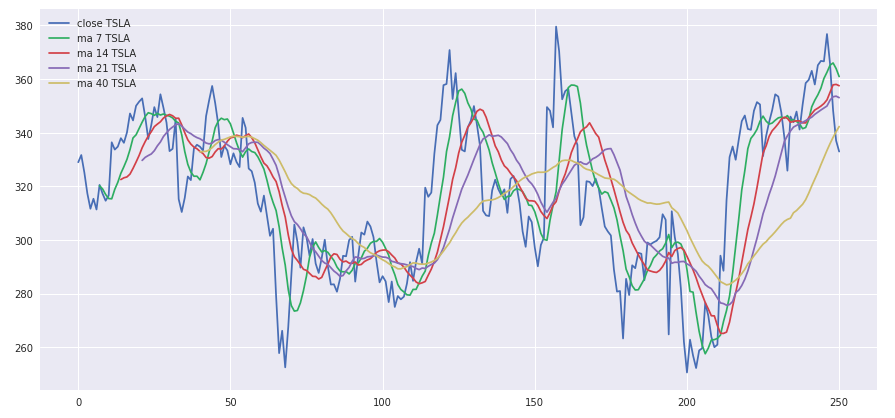
\includegraphics[width=\linewidth]{timeseries.png}
	\caption{Un insieme di TS, ciascuna di colore diverso}
	\label{fig:timeseries}
\end{figure}
Le TS consistono in una sequenza finita di \textit{osservazioni} periodiche fatte in un certo intervallo di tempo, ciascuna caratterizzata da uno o più valori discreti.\\
Il numero di osservazioni registrate nell'intervallo temporale definisce la cosiddetta \textbf{lunghezza} della time series, cioè la sua \textbf{dimensionalità}.\\
\\
L'\textbf{analisi delle time series} si occupa di studiare questi dati per estrarre informazioni statisticamente rilevanti per poi applicarle per diversi scopi:
\begin{itemize}
	\item \textbf{Previsioni}: prevedere l'andamento di alcuni eventi nel futuro, come ad esempio l'evoluzione delle azioni in borsa e le oscillazioni della Terra, tramite un \textit{modello statistico};
	\item \textbf{Stime}: approssimare le informazioni per ricavare conoscenza generale dei fenomeni analizzati;
	\item \textbf{Anomaly detection}: identificare e studiare la presenza di comportamenti anomali nei fenomeni analizzati.
\end{itemize}

I migliori risultati in questo ambito si ottengono nei task di:
\begin{itemize}
	\item \textbf{Classificazione}, che consiste nella costruzione di un modello di ML\footnote{Machine Learning} che apprende dalle TS il modo in cui assegnare ad una nuova TS una certa etichetta appartenente ad un insieme finito di classi. L'apprendimento è di tipo \textbf{supervisionato}.\\
	Tipicamente, i modelli usati per affrontare questo task sono basati su reti neurali ricorrenti, in particolare le \textbf{LSTM}, usate in questo lavoro e descritte nel seguito;
	
	\item \textbf{Clustering}, il cui obiettivo è quello di partizionare le serie temporali in gruppi, chiamati \textit{cluster}, a seconda della loro distanza in modo che le TS assegnate allo stesso cluster siano quanto più simili possibile. L'apprendimento è di tipo \textbf{non supervisionato}.\\
	Particolare attenzione va data alla scelta della metrica di similarità e dell'algoritmo di clustering: usare metriche e tecniche di clustering differenti potrebbe portare a risultati completamente diversi.\\
	In questo lavoro verrà usato l'algoritmo di clustering \textbf{k-Means}, con \textbf{distanza euclidea} come metrica di similarità, e verrà presentata un'altra soluzione che fa uso della distanza \textbf{DTW}\footnote{Dynamic Time Warping}, descritta nel seguito.
	
\end{itemize}
L'analisi di TS e la costruzione di un modello di ML devono affrontare problematiche specifiche per questo tipo di dati, ad esempio:
\begin{itemize}
	\item Ogni singola osservazione di una TS è memorizzata in una colonna del dataset, quindi una TS con un alto numero di osservazioni determina un forte aumento della sua dimensionalità, rendendo molto lunga la fase di training e creando modelli non sempre performanti\footnote{La cosiddetta \textbf{Curse of dimensionality}};
	\item E' difficile trovare una metrica di similarità che sia \textit{valida}, ovvero che restituisca un valore alto di similarità per le sole TS con andamenti realmente simili, ed \textit{efficiente}, ovvero che il suo tempo di calcolo risulti accettabile;
	\item Un dataset potrebbe contenere TS di \textbf{lunghezze differenti}, andando a complicare ulteriormente l'analisi per via del non allineamento di tutte le serie;
	\item Una singola osservazione può contenere più di un singolo valore discreto andando a complicare ulteriormente l'analisi per via della grande quantità di dati da elaborare.
\end{itemize}

Per risolvere il problema della dimensionalità, un buon approccio è quello di utilizzare tecniche di \textbf{feature extraction}, ovvero algoritmi che estraggono feature non note dalle TS, permettendo ai modelli di allenarsi su queste nuove feature piuttosto che sulle singole osservazioni.\\
Inoltre, è possibile anche applicare delle tecniche di \textbf{feature selection}, che selezionano solamente le feature rilevanti, andandone a ridurne di numero.\\
In maniera concettualmente simile, si potrebbe codificare l'input, ovvero la singola TS, in un formato "compresso", di dimensione ridotta ma che, allo stesso tempo, ne preservi le principali caratteristiche.\\
\\
Per risolvere il problema della metrica di similarità bisognerebbe usare ana funzione di distanza che tenga conto della natura delle TS e di tutte le loro particolarità.\\

\section{Il problema}
Il progetto è svolto in sinergia con altri gruppi e ha come obiettivo quello di confrontare approcci differenti per effettuare il \textbf{clustering} di TS, in modo da determinare la validità delle varie soluzioni.\\
Per il problema in questione sono stati assegnati vari dataset e ogni gruppo ha ricevuto l'incarico di determinare delle soluzioni valide e di evidenziarne i punti di forza e le debolezze. Ai fini di effettuare un'analisi comparativa adeguata, vengono usate alcune \textbf{misure di valutazione di clustering} comuni a tutte le soluzioni.

\section{Stato dell'arte}
L'analisi delle time series è uno dei principali campi di \textbf{ricerca} e sul quale si sta investendo maggiormente attualmente. Non sono pochi, infatti, i progetti nati negli ultimi anni che hanno contribuito allo sviluppo in merito.\\
\\
\textbf{TSFresh}\cite{tsfresh} è una libreria per \textit{Python}, compatibile con \textit{Scikit-Learn}, per l'estrazione automatica delle feature delle time series. La libreria permette di estrarre le caratteristiche rilevanti di una TS come la media, il valore minimo, il numero di picchi, la mediana, ecc.\\
La libreria, tra l'altro, assegna un \textit{valore di rilevanza} alle feature, così da permettere la selezione di quelle più rilevanti. Viene offerto anche un supporto al calcolo parallelo e distribuito.\\
L'estrazione e selezione delle feature permettono di superare i problemi discussi prima, su tutti quello della lunghezza differente delle serie temporali, rendendo l'analisi molto più precisa ed efficace.\\
TSFresh funziona solo come estrattore e selettore di feature, e non fornisce alcun modello di classificazione, regressione o clustering.\\
\\
\textbf{TSLearn}\cite{tslearn} è una libreria per Python scritta in \textit{C++} per l'analisi di time series. A differenza di TSFresh, essa offre, tra l'altro, dei modelli di ML ad hoc per le TS. E' in grado di leggere i dataset, di farne del preprocessing, di effettuare classificazione e regressione con SVM e clustering, usando metriche di distanza ad hoc per le TS, come il già citato DTW.\\
La libreria è piuttosto giovane (v:0.12.0) e sono pochi gli algoritmi implementati; anche la documentazione risulta poco curata nel dettaglio.

\section{Soluzione proposta}
Come approccio principale per affrontare il problema descritto, si è scelto di fare uso di un \textbf{autoencoder}, una particolare rete neurale in grado di codificare l'input, qui le TS, in una forma "compressa", chiamata \textbf{vettore latente}, ricavata rispetto agli iperparametri della rete.\\
Questa rappresentazione codificata dell'input viene usata per effettuare il clustering attraverso k-Means, non solo \textbf{reiterando l'esecuzione più volte per ottenere una maggiore precisione}, ma anche verificando la suddivisione \textbf{usando un diverso numero di cluster}.\\
Per ogni esecuzione di k-Means vengono mostrati i risultati tramite le misure di validazione di clustering in comune con gli altri gruppi.\\
\\
I risultati del clustering con l'autoencoder verranno confrontati con un \textbf{clustering basato su metrica DTW} tramite la libreria \textbf{TSLearn}.\\
Successivamente, il confronto verrà fatto con i risultati degli altri gruppi, che hanno fatto uso di clustering con \textbf{tecniche di feature extraction and selection} basate su \textbf{TSFresh} e altri algoritmi.\\
L'analisi comparativa ha lo di scopo di valutare le prestazioni sui soli dataset in esame e su determinate categorie di TS, cercando di dare un'idea di quali tecniche possano funzionare meglio e su quali tipologie di serie temporali.\\
\\
Per realizzare questo lavoro è stato scelto il linguaggio \textit{Python} per via dell'alto supporto fornito dalle sue libreria, quali \textit{Scikit-Learn}\cite{sklearn_api}, \textit{NumPy}\cite{numpy}, \textit{Matplotlib}\cite{matplotlib} e \textit{Pandas}\cite{pandas}. Il codice è stato sviluppato e curato con l'utilizzo di notebook \textit{Jupyter}, così da poter permettere una veloce ed efficace gestione del progetto: per le varie tecniche pensate è stato necessario valutarne la bontà con una prototipazione veloce e semplice che permettesse inoltre di rieseguire determinate porzioni di codice e mostrare graficamente i risultati ottenuti.\\

\section{Validazione della soluzione}
Per poter valutare le prestazioni dell'autoencoder si adotteranno alcune \textbf{misure interne} e \textbf{misure esterne}\cite{metrics} di valutazione di clustering. Esse saranno usate per questi scopi:
\begin{itemize}
	\item Valutare la \textbf{bontà del modello} proposto e il \textbf{valore ottimale dei suoi iperparametri};
	\item Valutare \textbf{l'efficacia dell'algoritmo k-Means};
	\item Valutare il \textbf{numero ottimale di cluster} per k-Means;
	\item Valutare la \textbf{qualità dei dataset in esame}.
\end{itemize}
Le misure sono anche dette \textbf{indici}.

\subsection{Misure di validazione interne}
Una \textbf{misura di validazione interna} si occupa di validare i risultati di un algoritmo di clustering guardando quanto bene ha accomunato (messi in uno stesso cluster) item simili e quanto bene ha separato (messi in cluster diversi) item differenti.\\
In altre parole, si vuole minimizzare la distanza intra-cluster e massimizzare la distanza inter-cluster\footnote{Queste distanze sono calcolate a seconda della metrica di distanza scelta}.\\
\\
La \textbf{compactness} (o cohesion) misura quanto bene sono vicini gli item in ciascun cluster ed è, tipicamente, la somma dei quadrati di tutte le distanze degli item di un cluster dal relativo centroide. E' bene minimizzarla il più possibile.\\
La \textbf{separation} misura quanto bene sono distanziati gli item in diversi cluster ed è, tipicamente, la somma dei quadrati di tutte le distanze tra tutti i centroidi. E' bene massimizzarla il più possibile.\\
\textbf{Le misure di interne sono basate sui concetti di compactness e separation}.\\
\\
E' bene ricordare che alcuni algoritmi di clustering già hanno come scopo quello di ottimizzare uno solo dei due aspetti oppure entrambi, quindi potrebbe capitare che alcune misure risultino quasi sempre alte se si applica un determinato algoritmo, altre quasi sempre basse.

\subsubsection{Silhouette Coefficient}
Il \textbf{Silhouette Coefficient di un item $i$}, o semplcemente la \textit{silhouette}, serve a stabilire quanto bene $i$ è stato assegnato al giusto cluster.\\
\\
Sia $i$ un'item e sia $d$ una qualsiasi funzione di distanza. Il Silhouette Coefficient di i, $S(i)$ si calcola nel seguente modo:
\begin{align}
S(i) = \frac{b_i - a_i}{max(a_i, b_i)}
\end{align}
dove:
\begin{enumerate}[(i)]
	\item $$ a_i = \frac{1}{|C|-1}\sum_{i\ne j\in C} d(i,j)$$ è la distanza media dell'item i rispetto agli altri item j nello stesso cluster C.\\
	Più il valore è piccolo, più l'item i è vicino agli altri item dello stesso cluster;
	\item $$ b_i = \min_{k\ne i} \frac{1}{|C_k|}\sum_{j \in C_k} d(i,j)$$ è la distanza media dell'item i rispetto agli item j nel più vicino cluster\footnote{Anche detto \textit{neighbour cluster}} diverso da quello che contiene i.
\end{enumerate}
E' compreso tra -1 e 1, con -1 indicante un clustering totalmente errato, 1 indicante un clustering altamente denso e ben separato e 0 indicante clustering sovrapposti (il caso medio).\\
Si osserva che se $b_i > a_i$, allora $S(i)$ risulterà compreso tra -1 e 0, sintomo di un'assegnazione di $i$ al cluster sbagliato: sarebbe più opportuno assegnarlo al cluster più vicino.\\
Se $b_i < a_i$, allora $S(i)$ risulterà compreso tra 0 e 1. Più $a_i$ tende a 0, più $S(i)$ tenderà ad 1, sintomo di perfetta assegnazione di $i$ al cluster giusto.\\
Se $S(i)$ è circa 0 allora l'item non dovrebbe stare in nessuno dei due cluster proposti, e sarebbe quindi opportuno rivalutare il numero di cluster scelti, se non proprio l'algoritmo di clustering stesso.\\
\\
E' possibile calcolare il Silhouette Coefficient medio di tutto il clustering. Sia D l'insieme di tutti gli item:
\begin{align}
S = \frac{1}{|D|} \sum_{i \in D} S(i)
\end{align}
Più S tende ad 1, migliore è l'assegnazione degli item.\\
La sua elaborazione può richiedere molto tempo se la metrica di distanza è complessa.

\subsubsection{Davies-Bouldin Index}
Il \textbf{Davies-Bouldin Index} (DB) di un clustering misura la media di similarità di ciascun cluster con il suo cluster più simile.\\
\\
Sia m il numero di cluster, il Davies-Bouldin Index è calcolabile nel seguente modo:
\begin{align}
DB = \frac{1}{m}\sum_{i=1}^{m}\max_{i \ne j}sim(C_i, C_j)
\end{align}
dove:
\begin{enumerate}[(i)]
	\item $$ sim(C_i, C_j) =  \frac{c_i + c_j}{d(C_i, C_j)}$$ è una misura di \textit{similarità tra due cluster}.\\
	$c_i$ è la compactness del cluster $C_i$ calcolata come distanza media di tutti gli item in $C_i$ rispetto al proprio centroide.\\
	$d(C_i, C_j)$ è la separation tra i cluster $C_i$ e $C_j$, calcolata come distanza tra i rispettivi centroidi.
\end{enumerate}
Ha 0 come lower bound e, a differenza di altri indici, un buon clustering è rappresentato da un DB tendente a 0. Per minimizzare DB, bisogna rendere i cluster il meno simili possibile, minimizzando le compactness di ciascun cluster (i valori $c_i$) oppure massimizzando la separation tra cluster ($d(C_i, C_j)$).\\
Cluster molto densi e distanti hanno DB minimo. Con \textit{DBSCAN} si raggiungono quasi sempre score tendenti a 0 poiché l'algoritmo ottimizza la densità dei singoli cluster.

\subsubsection{Altre misure interne}
Non esistono molte altre misure interne affermate, ma è bene citare il \textbf{Dunn Index} che misura quanto bene i cluster siano compatti e separati l'uno dall'altro.\\
\\
Sia m il numero di cluster, il Dunn Index è calcolabile nel seguente modo:
\begin{align}
D = \frac{\min_{1\le i \le j \le m}\delta(C_i, C_j)}{\max_{1 \le k \le m}(diam(C_k))}
\end{align}
dove:
\begin{enumerate}[(i)]
	\item $ \delta(C_i, C_j) $ è la separation tra due cluster $C_i$ e $C_j$, calcolata attraverso una qualsiasi metrica di distanza.\\
	Il numeratore di D considera la più piccola di queste separazioni, escludendo quelle già calcolate;
	\item $ diam(C_k) $ è una funzione che calcola il \textit{diametro} del cluster $C_k$, ovvero la massima distanza (di qualsiasi tipo) tra due dei suoi item. E' una particolare misura di compactness.
\end{enumerate}
Cluster molto grandi hanno una maggiore probabilità di avere un diametro maggiore, e quindi una maggiore probabilità di aumentare il denominatore di $D$, andando a diminuire l'indice. Aumentare di molto il numero di cluster andrà ad aumentare $D$ con alta probabilità.\\
E' un indice rilevante in dataset molto grandi e/o quando è previsto avere un grande numero di cluster.

\subsection{Misure di validazione esterne}
Una \textbf{misura di validazione esterna} si occupa di validare i risultati di un algoritmo di clustering rispetto a delle \textbf{ground truth}\footnote{Verità di base}, ovvero delle informazioni relative ad un altro tipo di clustering o ad una classificazione degli stessi dati non usata per compiere il clustering in valutazione.\\
Nelle ground truth, quindi, \textbf{ogni item possiede una classe} (o label), da usare come oracolo.\\
\\
A differenza delle misure interne, che si pongono di misurare cluster compatti e separati, \textbf{le misure esterne misurano la \textit{fedeltà} dei cluster alle ground truth}. La fedeltà è spesso calcolata tramite il \textbf{pair counting}\footnote{Conteggio delle coppie}, ovvero contando:
\begin{itemize}
	\item Il numero di coppie di item clusterizzati insieme se essi sono della stessa classe. Anche detto numero di \textbf{True Positive} (TP);
	\item Il numero di coppie di item clusterizzati insieme se essi sono in classi diverse. Anche detto numero di \textbf{False Positive} (FP);
	\item Il numero di coppie di item NON clusterizzati insieme se essi sono della stessa classe. Anche detto numero di \textbf{False Negative} (FN);
	\item Il numero di coppie di item NON clusterizzati insieme se essi sono in classi diverse. Anche detto numero di \textbf{True Negative} (TN);
\end{itemize}
Chiaramente, come nel task della classificazione, lo scopo generale è quello di massimizzare TP e TN e di minimizzare FP e FN.\\
Molti degli indici esterni sono, quindi, \textbf{basati su conteggi non pesati}, che assegnano un peso uguale a tutte le diverse tipologie di coppie.

\subsubsection{Contingency Matrix}
La \textbf{Contingency Matrix}, più che un vero e proprio indice, è una matrice che riporta la cardinalità delle intersezioni dei cluster con tutte le classi delle ground truth. L'elemento $x_{ij}$ rappresenta il numero di item della classe $i$ presenti nel cluster $j$.\\
Quanti più valori tendenti a 0 possiene una colonna, tanto più quel cluster è fedele ad una delle classi. Se il numero di cluster è uguale al numero di classi ($i=j$), è bene che un cluster ne ricopra una e una sola.\\
\begin{table}[H]
	\centering
	\begin{tabular}{c | c c c c}
		& $A_1$ & $A_2$ & $...$ & $A_m$\\
		\hline
		$B_1$ & $x_{11}$ & $x_{12}$ & $...$ & $x_{1m}$\\
		$B_2$& $x_{21}$ & $x_{22}$ & $...$ & $x_{2m}$\\
		$...$ & $...$ & $...$ & $...$ & $...$\\
		$B_n$& $x_{n1}$ & $x_{n2}$ & $...$ & $x_{nm}$
	\end{tabular}
	\caption{Contingency Matrix che confronta un labelling di n classi e un clustering di m cluster. $x_{ij}$ è il numero di item della classe $i$ presenti nel cluster $j$}
	\label{tab:contingency}
\end{table} 
Non essendo un valore scalare, risulta di difficile interpretazione se il numero di cluster e/o di classi aumenta molto. Allo stesso tempo, è molto utile per dare una prima interpretazione della fedeltà del clustering rispetto alle ground truth.

\subsubsection{Purity}
La \textbf{Purity} è una misura che stabilisce quanto bene un clustering copra le ground truth. Precisamente, misura quanto un cluster contiene elementi di una singola classe.\\
\\
Formalmente, sia C il clustering analizzato, L l'insieme di classi di riferimento, e sia N l'insieme degli item:
\begin{align}
P = \frac{1}{|N|}\sum_{c \in C}\max_{l \in L}|c \cap l|
\end{align}
E' compresa tra 0 e 1, con 0 indicante nessuna copertura, e 1 indicante copertura massima.\\
Ogni cluster partecipa alla sommatoria con il numero di item della classe assolutamente più diffusa al suo interno. Guardando alla Contingency Matrix, si sommano i valori massimi di ciascuna colonna.\\
\\
Non è consigliata con classi sbilanciate poiché risulterà facilmente alta per via dell'alta probabilità che un cluster abbia come classe più diffusa quella massima.\\
Per ridurre questo effetto negativo si potrebbe pensare di considerare il massimo relativo di ciascun cluster invece che del massimo assoluto: ogni cluster partecipa alla sommatoria con il numero di item della classe relativamente più diffusa al suo interno.\\
La divisione viene comunque fatta sul numero totale di elementi. Questa misura può essere chiamata \textbf{Relative Purity}, anche essa compresa tra 0 e 1 e con identico significato.

\subsubsection{Rand index e Adjusted Rand index}
Il \textbf{Rand index} (RI), o \textbf{Accuracy}, è il rapporto tra il numero di coppie correttamente clusterizzate (ottenuto dalla somma di TP e TN) sul numero di coppie non ordinate totali.\\
Sia n il numero di item, il Rand Index si calcola nel seguente modo:
\begin{align}
RI = \frac{TP + TN}{C_2^n}
\end{align}
Il numero di coppie non ordinate può anche essere calcolato sommando TP, FP, FN e TN.\\
E' compreso tra 0 e 1, dove 0 indica che il clustering e il labelling non concordano su alcun punto, mentre 1 indica che c'è concordanza massima.\\
\\
Il Rand index presenta un problema grave: valutare un \textit{clustering casuale uniforme}, anche detto \textbf{random labelling}, rispetto ad ground truth determina sempre un buon valore, crescente con il numero di cluster creati. Chiaramente questa situazione non è desiderabile, ed è casuata dal fatto che i quattro valori pesano tutti allo stesso modo sul risultato.\\
Per risolvere questo problema si usa una versione "aggiustata" dell'indice, chiamata \textbf{Adjusted Rand Index} (ARI)\cite{ari}.\\
L'ARI tiene conto del RI del random labelling e lo usa come riferimento:
\begin{align}
ARI = \frac{RI - E[RI]}{max(RI) - E[RI]}
\end{align}
dove:
\begin{enumerate}[(i)]
	\item $ RI $ è il Rand index calcolato al solito modo;
	\item $ E[RI] $ è il valore atteso del Rand Index, calcolabile con la formula del valore atteso di una variabile aleatoria ipergeometrica (il Rand Index può essere modellato come ipergeometrica) oppure calcolando il RI di un clustering uniforme casuale;
	\item $ max(RI) $ è il massimo valore che può assumere il Rand Index, calcolato come media del numero di coppie di item di ciascun cluster e di ciascuna classe.
\end{enumerate}
E' compreso tra -1 e 1, dove -1 indica che il clustering è paragonabile ad un clustering casuale rispetto al labelling, mentre 1 indica match perfetto.\\

\subsubsection{Pairwise Precision, Recall, F1-Score e Fowlkes-Mallows index}
Precision, Recall ed F1-Score sono misure molto usate nel task di classificazione, e possono essere riproposte anche nel clustering se considerate nella loro versione pairwise, cioè che contano il numero di coppie invece che i singoli item.\\
La \textbf{Precision} di un clustering rispetto a delle ground truth è calcolata nel seguente modo:
\begin{align}
Pr = \frac{TP}{TP + FP}
\end{align}
La \textbf{Recall} di un clustering rispetto a delle ground truth è calcolata nel seguente modo:
\begin{align}
Re = \frac{TP}{TP + FN}
\end{align}
L'\textbf{F1-Score} di un clustering rispetto a delle ground truth è la media armonica di Precision e Recall; calcolata nel seguente modo:
\begin{align}
F_1 = 2\:\frac{Pr * Re}{Pr + Re}
\end{align}
Il \textbf{Fowlkes-Mallows index} (FMI), o \textbf{G-Measure}, di un clustering rispetto a delle ground truth è la media geometrica di Precision e Recall; calcolato nel seguente modo:
\begin{align}
FM = \sqrt{Pr * Re}
\end{align}
Tutte e quattro le misure sono comprese tra 0 e 1, con 0 indicante totale indipendenza tra clustering e labelling, e con 1 indicante match perfetto.\\
Il Fowlkes-Mallows è immune al random labelling: in quel caso ritorna uno score tendente a 0.\\
Nessuna delle quattro misure tiene conto dei TN, cosa che potrebbe essere utile in alcuni casi.

\subsubsection{Altre misure esterne}
Esistono numerose altre misure esterne, tra le quali:
\begin{itemize}
	\item \textbf{Homogeneity}, misura quanto un cluster contenga item di una singola classe;
	\item \textbf{Completeness}, misura quanto gli item di una classe appartengano allo stesso cluster;
	\item \textbf{V-Measure}, media armonica tra Homogeneity e Completeness. Non è immune al random labelling;
	\item \textbf{Jaccard index}, basata sulla similarità di Jaccard ed è il rapporto tra TP e la somma di TP, FP e FN;
	\item \textbf{Dice index}, come il Jaccard, ma da un peso doppio alle coppie TP;
	\item \textbf{Mutual Information Score}, basati sulle misure della teoria dell'informazione, come l'entropia. Misura l'informazione condivisa tra il clustering e il labelling usando similarità non lineari (logaritmiche).\\
	Non essendo immune al random labelling, si usano spesso la \textbf{Normalized Mutual Information Score} e la \textbf{Adjusted Mutual Information Score}.
\end{itemize}

\section{Struttura del documento}
Nel capitolo \ref{chap:dataset} verranno presentati i dataset scelti per valutare la soluzione proposta, illustrandone le caratteristiche principali.\\
\\
Nel capitolo \ref{chap:solution} verrà presentata la soluzione proposta, ovvero quella che ricorre all'uso di un autoencoder. Nello stesso capitolo verranno anche mostrati i risultati del modello.\\
\\
Nel capitolo \ref{chap:comparison} verranno confrontati i risultati dell'autoencoder con il clustering con DTW di TSLearn e con il clustering degli altri gruppi.\\
\\
Infine, nel capitolo \ref{chap:conclusioni} verranno tratte le conclusioni riguardanti l'autoencoder, i dataset in esame e l'algoritmo di clustering scelto.\\